%%%%%%%%%%%%%%%%%%%%%%%%%%%%%%%%%%%%%%%%%%%%%%%%%%%%%%%%%%%%%%%%%%%%%%%
%
%   Presentation of Beamer UNL Theme
%   Beamer Presentation by Chris Bourke
%
%%%%%%%%%%%%%%%%%%%%%%%%%%%%%%%%%%%%%%%%%%%%%%%%%%%%%%%%%%%%%%%%%%%%%%%

% \documentclass[mathserif]{beamer}
\documentclass[10pt,aspectratio=169]{beamer}
% \usepackage[english]{babel}
\usetheme[outer/progressbar=foot,
outer/numbering=fraction]{metropolis}

% \usetheme[hideothersubsections]{UNLTheme}
% \usetheme{Boadilla}
% \usecolortheme{seagull}

\usepackage{graphicx}
\usepackage{wrapfig}
\usepackage{natbib}
\usepackage{amsmath}
\usepackage{pifont}
\usepackage{mathtools} % Math packages
\usepackage{hyperref}% add hypertext capabilities
\usepackage{caption}
\usepackage{subcaption}
\usepackage[multidot]{grffile}
\usepackage[capitalise]{cleveref}
\crefname{eq:}{Eq.}{Eqs.}
\crefname{fig:}{Fig}{Figs}
\usepackage{tikz,tikz-3dplot}
\usepackage{pgfplots}
\usetikzlibrary{arrows,shapes}
% \tikzstyle{every picture}+=[remember picture]
% By default all math in TikZ nodes are set in inline mode. Change this to
% displaystyle so that we don't get small fractions.
\everymath{\displaystyle}

% transparency
\setbeamercovered{transparent=15}

\title[Recent advances in simulation of B in galaxies]{Recent advances in simulation of magnetic fields in galaxies}
\author[S.Mohammad Hosseinirad]
{S.Mohammad Hosseinirad} %
\institute[FUM]{Ferdowsi Univ. of Mashhad\\ Journal club meeting}
\date{23 Aban 99}
%\titlegraphic{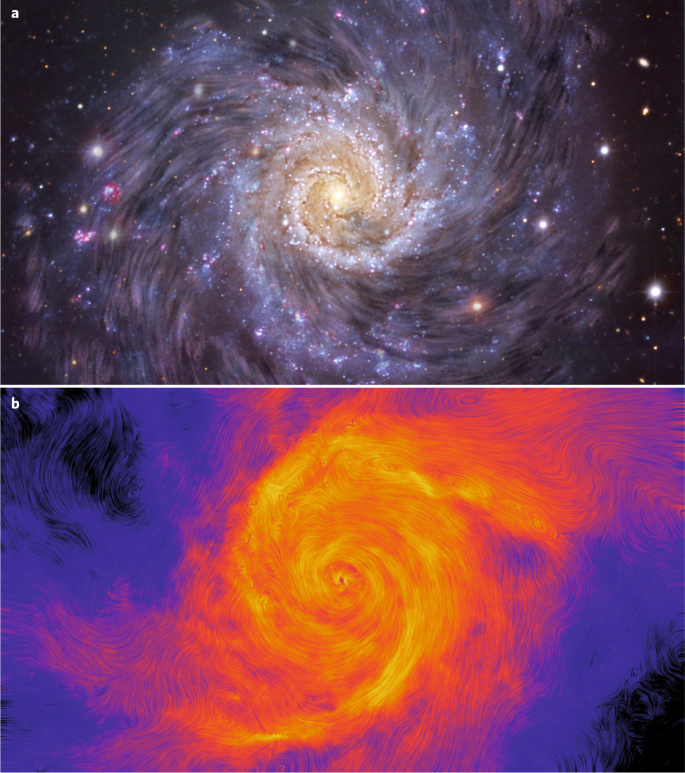
\includegraphics[width=2cm]{images/1.png}} 
%%% new commands
\newcommand{\ds}{\displaystyle}
\newcommand{\be}{\begin{equation*}}
\newcommand{\ee}{\end{equation*}}
\newcommand{\bvec}[1]{{\bf #1}}
\newcommand{\recip}[1]{\frac{1}{#1}}
\newcommand{\tpartial}[1]{\frac{\partial\, #1}{\partial t}}
\newcommand{\pidrv}[1]{\frac{d\, #1}{d\varpi}}
\newcommand{\piddrv}[1]{\frac{d^{2}\, #1}{d\varpi^{2}}}
\newcommand{\kk}{k^{2}}
\newcommand{\ww}{\omega^{2}}
\newcommand{\BB}{B^{2}}
\newcommand{\cs}{c_{\rm s}}
\newcommand{\rhoc}{\rho_{\rm c}}
\newcommand{\pcc}{\mbox{ cm$^{-3}$}}
\newcommand{\gpcc}{\mbox{ g cm$^{-3}$}}
\newcommand{\kms}{\mbox{ km sec$^{-1}$}}
\newcommand{\kfast}{k_{\rm fast}}
\newcommand{\lfast}{\lambda_{\rm fast}}
\newcommand{\wfast}{|\omega_{\rm fast}|}
\newcommand{\pp}[2]{\frac{\partial\, #1}{\partial\, #2 }}
\newcommand{\dr}[1]{\dfrac{d #1}{dr}}
% \newcommand{\dz}[1]{\dfrac{d #1}{dz}}
\newcommand{\ex}{e^{i(kz-\omega t)}}

\setbeamerfont{caption}{size=\scriptsize}
%%%%%%%%%%%%%%
\begin{document}

%{% open a Local TeX Group
%\setbeamertemplate{sidebar}{}
\begin{frame}
        \titlepage
%         \begin{center}
%     \href{mailto:m.rad@birjand.ac.ir}{\color{blue}{\texttt{m.rad@birjand.ac.ir}}}
%         \end{center}
\end{frame}
%}% end Local TeX Group

%........................................................
%........................................................
\section{Magnetic field}
%........................................................
%........................................................
\begin{frame}
\frametitle{Importance of magnetic field}
	\begin{columns}
		\begin{column}{0.55\textwidth}
			\begin{itemize}%[<+->]
				\item B is omnipresent in the universe and observed on vastly different scales
				\item In galaxies B is specially important
				\begin{itemize}
					\item Magnetic pressure in the ISM is comparable to the thermal pressure
					\item B determines the propagation of cosmic rays
				\end{itemize}
			\end{itemize}
		\end{column}
		\begin{column}{0.45\textwidth}
			\begin{figure}
				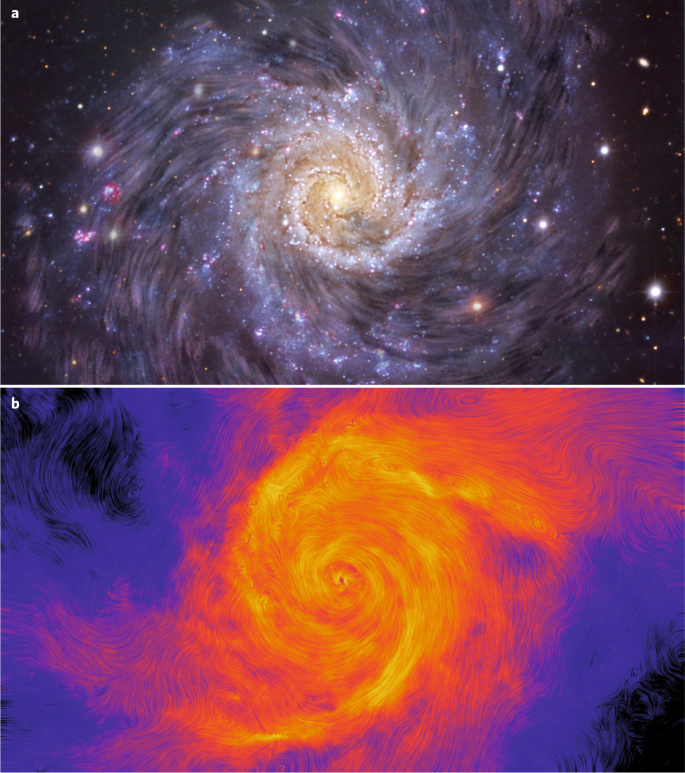
\includegraphics[width=6cm,trim=40 50 5 30,clip]{./images/1.png}
				\caption{Galactic magnetic fields from observations (NGC 628) and simulations. Credit: top, Mulcahy et al. (2017); bottom, courtesy of Pakmor.}
			\end{figure}
		\end{column}
	\end{columns}
\end{frame}
%........................................................
\begin{frame}
\frametitle{MHD}
	\begin{align}
		\frac{\partial \rho}{\partial t} + \nabla\cdot\left(\rho\bvec{v}\right) = 0
	\end{align}
	\begin{align}
		\rho\frac{\partial \mathbf{v}}{\partial t} + \rho\left(\bvec{v}\cdot\nabla\right) \bvec{v}
		+ \nabla p + \rho\nabla\psi
		- \dfrac{1}{4\pi}\left(\nabla\times\bvec{B}\right)\times\bvec{B} = 0,
	\end{align}
	\begin{align}
		\frac{\partial \mathbf{B}}{\partial t} &= \nabla \times \left( \mathbf{v} \times \mathbf{B} \right) \\
		&= (\mathbf{B} . \nabla) \mathbf{v} - \mathbf{B}(\nabla . \mathbf{v}) + \mathbf{v}(\nabla . \mathbf{B}),
	\end{align}
	\begin{equation}
		\nabla^{2}\psi = 4\pi G \rho.
	\end{equation}
\end{frame}
%====================
\begin{frame}
	\frametitle{Building up magnetic fields}
	\begin{itemize}
		\item seeding
		\item amplifying and sustaining
%		\item ordering
%		\item sustaining
	\end{itemize}
\end{frame}
%====================
\begin{frame}
	\frametitle{Seeding}
	\begin{itemize}
		\item Seed fields can be "primordial", i.e. generated in the early Universe (Durrer $\&$ Neronov 2013)
		\item May originate from later epochs, e.g. during cosmological structure formation by the Weibel instability (Lazar et al. 2009)
		\item Plasma fluctuations in protogalaxies (Schlickeiser 2012; Schlickeiser $\&$ Felten 2013)
		\item The Biermann mechanism in the first SN remnants (Hanayama et al. 2005)
	\end{itemize}
\end{frame}
%====================
\begin{frame}
	\frametitle{Amplifying}
	\begin{itemize}
		\item An efficient source of field amplification is the turbulence driven by SN explosions (Ferrière 1996) or by spiral shocks (Kim et al. 2006), called the \textbf{small-scale dynamo}.
	\end{itemize}
	In protogalaxies this mechanism can amplify weak seed fields to several $\mu G$ strength (the energy level of turbulence) within less than $10^8$ year (Kulsrud et al. 1997; Schleicher et al. 2010; Beck et al. 2012a; Rieder $\&$ Teyssier 2015). The resulting field is turbulent.
\end{frame}
%====================
%\begin{frame}
%	\frametitle{Ordering}
%	The final and most time-consuming stage is the \textbf{ordering} of the turbulent field.
%	\begin{itemize}
%		\item Numerical models of evolving galaxies show fast field amplification and ordering with help of differential rotation (Wang $\&$ Abel 2009; Kotarba et al. 2009), possibly supported by the magneto-rotational instability (MRI) (Gresseletal. 2013; Pakmor $\&$ Springel 2013).
%		\item In these models the ordered magnetic field forms spiral arm segments, but it has frequent reversals in azimuthal and radial directions and hence is \textbf{anisotropic turbulent}.
%	\end{itemize}
%\end{frame}
%====================
\begin{frame}
	\frametitle{Sustaining}
	The most promising mechanism to \textit{sustain} magnetic fields and generate large-scale regular fields from turbulent fields in the ISM of galaxies is the \textbf{$\alpha-\Omega$} \textbf{dynamo} (Beck et al. 1996). It is based on 
	\begin{itemize}
		\item differential rotation ($\Omega$)
		\item $\alpha$-effect, cyclonic motion of turbulent gas flows by Coriolis force which are driven by stellar winds and SN explosions (Ferrière 1996; Gressel et al. 2013) or cosmic rays (Hanasz et al. 2009)
		\item magnetic diffusivity ($\eta$)
	\end{itemize}
\end{frame}
%====================
\begin{frame}
	\frametitle{The "mean-field" dynamo equation}
	Remember induction equation
	\begin{align}
	\frac{\partial \mathbf{B}}{\partial t} &= \nabla \times \left( \mathbf{V} \times \mathbf{B} \right) + \eta \nabla^2 \mathbf{B}
	\end{align}
	\begin{itemize}
		\item Represent $\mathbf{B}$ and $\mathbf{V}$ each as a sum of a slowly-varying mean field and a weak small-scale fluctuation component
	\end{itemize}
	\begin{align}
		\mathbf{B} = \langle \mathbf{B} \rangle + \mathbf{B}'
	\end{align}
	\begin{align}
	\mathbf{V} = \langle \mathbf{V} \rangle + \mathbf{V}'
	\end{align}
\end{frame}
%====================
\begin{frame}
	\frametitle{The "mean-field" dynamo equation} 
	\begin{align}
	\frac{\partial \mathbf{B}}{\partial t} &= \nabla \times \left( \mathbf{V} \times \mathbf{B} \right) + \nabla \times \alpha \mathbf{B} 
	+ (\beta+\eta) \nabla^2 \mathbf{B}
	\end{align}
	\begin{itemize}
		\item $\mathbf{B}$ and $\mathbf{V}$ are the mean magnetic field and velocity (usually rotational)
		\item $\beta$ can be interpreted as turbulent resistivity
	\end{itemize}
\end{frame}
%====================
\begin{frame}
	\frametitle{Schematic view} 
		\begin{figure}
			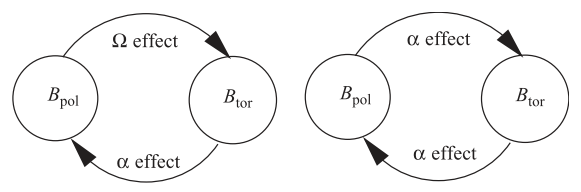
\includegraphics[width=0.75\textwidth]{./images/alpha_omega.png}
			\caption{Mutual regeneration of poloidal and toroidal fields in the case of the $\alpha-\Omega$ dynamo (left) and the $\alpha^2$ dynamo (right) (Brandenburg $\&$ Subramanian 2005).}
		\end{figure}
	\end{frame}
%........................................................
%........................................................
\section{Example works for isolated galaxies}
%........................................................
%........................................................
%====================
%\begin{frame}
%	\frametitle{SPH simulations of magnetic fields in galaxy clusters (Dolag et al. 1999)}
%%	\begin{center}
%%		\includegraphics[width=1\textwidth]{./images/dolag1999.png}
%%	\end{center} 
%		The first self-consistent simulations which follow the B amplification during the formation of galaxy clusters with cosmological environment
%\\\
%		\begin{itemize}
%			\item GrapeSPH (Steinmetz 1996) + B
%			\item A small initial magnetic seed field exists before structure formation
%			\item no cleaning for $\nabla \cdot B$
%		\end{itemize} 
%\end{frame}
%====================
%\begin{frame}
%	\frametitle{SPH simulations of magnetic fields in galaxy clusters (Dolag et al. 1999)}
%	\begin{itemize}
%		\item These runs were able to demonstrate that the contribution to the \textbf{amplification} of B by \textbf{shear} flows (and by its induced turbulence) is \textbf{significant}.
%		\item They showed that the \textbf{final structure of B} in a galaxy cluster is \textbf{determined by the structure formation} process, not by the initial B configuration.
%		\item Good prediction of today observed B in galaxy clusters from seeds at high redshift (z $\approx$ 3 and higher)
%	\end{itemize}
%	These results were confirmed by extending Gadget2 to follow the full set of ideal MHD equations (Dolag et al. 2004, 2005) even at much higher resolution.
%\end{frame}
%====================
\begin{frame}
	\frametitle{Simulations of magnetic fields in isolated disc galaxies \citep{2013MNRAS.432..176P}}
	\begin{itemize}
		\item AREPO code 
		\item SN feedback with a modified equation of state
		\item Powel et al. (1999) scheme for divergence cleaning. In this approach, additional source terms are introduced into the momentum, induction and energy equations, without modifying MHD solver, to keep errors as small as possible.
	\end{itemize}
Another method e.g.: 

- constrained transport approach (Evans $\&$ Hawley 1988). This methods is existed just for Cartesian grids and tries to avoid divergence error by construction.

- Dedner et al. (2002) in which a local divergence error is both advected away from the place where it originates and damped at the same time.
\end{frame}
%====================
\begin{frame}
	\frametitle{Simulations of magnetic fields in isolated disc galaxies (PV13)}
	\begin{columns}
		\begin{column}{0.55\textwidth}
			\begin{figure}
				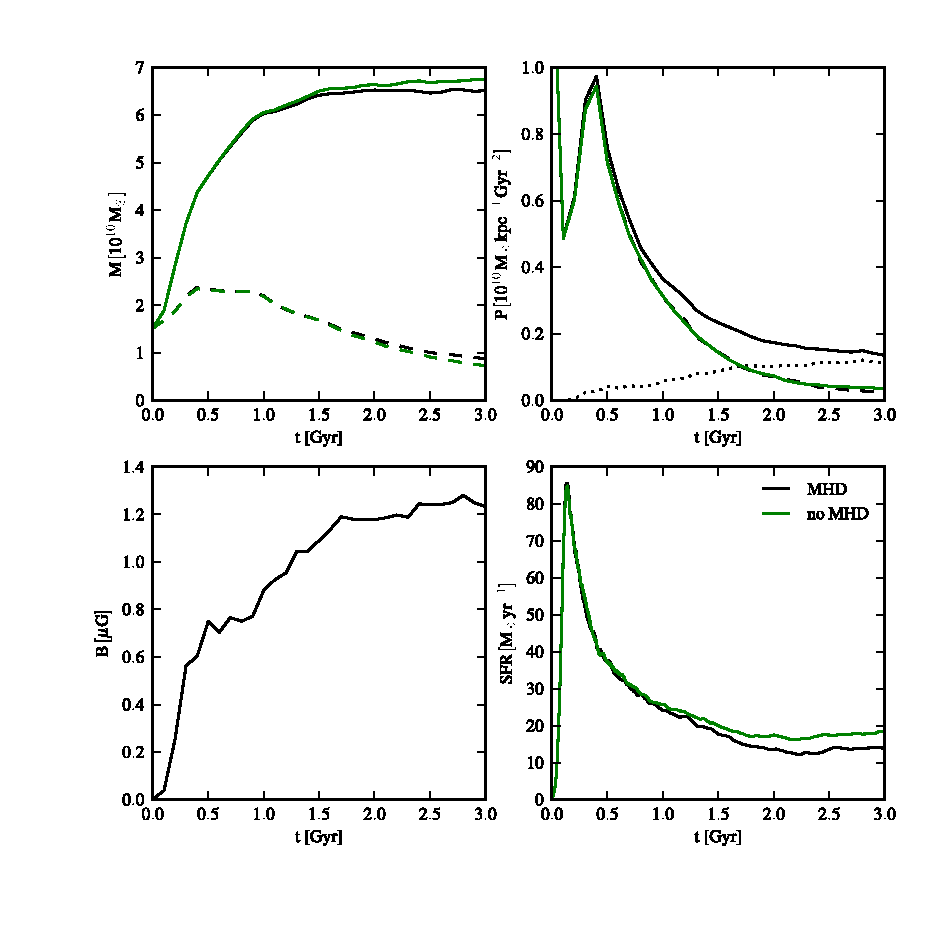
\includegraphics[width=7cm,trim=40 50 5 30,clip]{./images/timedepCmp.pdf}
				\caption{Time evolution of different quantities of a
					$10^{12}\,\mathrm{M_\odot}$ galaxy .}
			\end{figure}
		\end{column}
		\begin{column}{0.48\textwidth}
			
			- TL: total	baryonic mass in stars and gas (straight line) and the gas mass within a radius of $15\,\mathrm{kpc}$ (dashed line). 
			
			- TR: thermal pressure (dashed line), the magnetic pressure (dotted line) and the total pressure (straight line).
			
			- BL: magnetic field within a radius of $15\,\mathrm{kpc}$. 
			
			- BR: total star formation rate in the whole simulation
		\end{column}
	\end{columns}
\end{frame}
%====================
\begin{frame}
	\frametitle{Simulations of magnetic fields in isolated disc galaxies (PV13)}	
	\begin{itemize}
		\item B strength is \textbf{quickly amplified} in the initial central starburst and the differential rotation of the forming disc, eventually reaching a \textbf{saturation} value.
		\item At this point, the B pressure in the interstellar medium becomes comparable to the
		thermal pressure, and a further efficient growth of the B strength is prevented.
		\item B also leads to a \textbf{lower star formation rate} at late times compared to simulations without Bs, and induces changes in the spiral arm structures of the gas disc. 
		\item They observed highly magnetized fountain-like outflows from the disc.
		\item They argue that their results are robust with numerical resolution and are largely independent of the initial magnetic seed field strength assumed, as the amplification process is rapid and self-regulated.
	\end{itemize}
\end{frame}
%====================
%\begin{frame}
%	\frametitle{Magnetic fields in cosmological simulations of disk galaxies (Pakmor et al. 2014)}
%	\begin{itemize}
%		\item For the first time the formation and evolution of a Milky Way–like disk galaxy in its \textbf{full cosmological context} while taking into account B.
%		\item They found that a prescribed tiny magnetic seed field \textbf{grows exponentially} by a small-scale dynamo until it saturates around z = 4 with a magnetic energy of about $10\%$ of the kinetic energy in the center of the galaxy's main progenitor halo.
%		\item By z=2, a well-defined gaseous disk forms in which B is further \textbf{amplified} by differential rotation, until it saturates at an average field strength of $\sim 6 \mu G$ in the disk plane.
%		\item In this phase, B is transformed from a chaotic small-scale field to an \textbf{ordered} large-scale field on scales comparable to the disk radius.
%		\item They suggested that the \textbf{large-scale B in spiral galaxies} can be explained as a result of the \textbf{cosmic structure formation} process.
%	\end{itemize}
%\end{frame}
%====================
\begin{frame}
	\frametitle{Ab Initio Simulations of a Supernova-driven Galactic Dynamo in an Isolated Disk Galaxy \citep{2017ApJ...843..113B}}
		\begin{columns}
			\begin{column}{0.55\textwidth}
				\begin{itemize}
					\item ENZO code
					\item Dedner et al. (2002) $\nabla \cdot B$ cleaning
					\item initially unmagnetized galactic disk
					\item novel prescription for MHD SN feedback
					\item supernova events occur in proportion to star formation activity and provide localized injections of thermal energy, metal-rich material, and a low level of toroidal B
					\item neglect the influence of CRs and focus on the role of turbulence driven by supernovae through their thermal feedback.
				\end{itemize}
			\end{column}
			\begin{column}{0.48\textwidth}
			\begin{figure}
				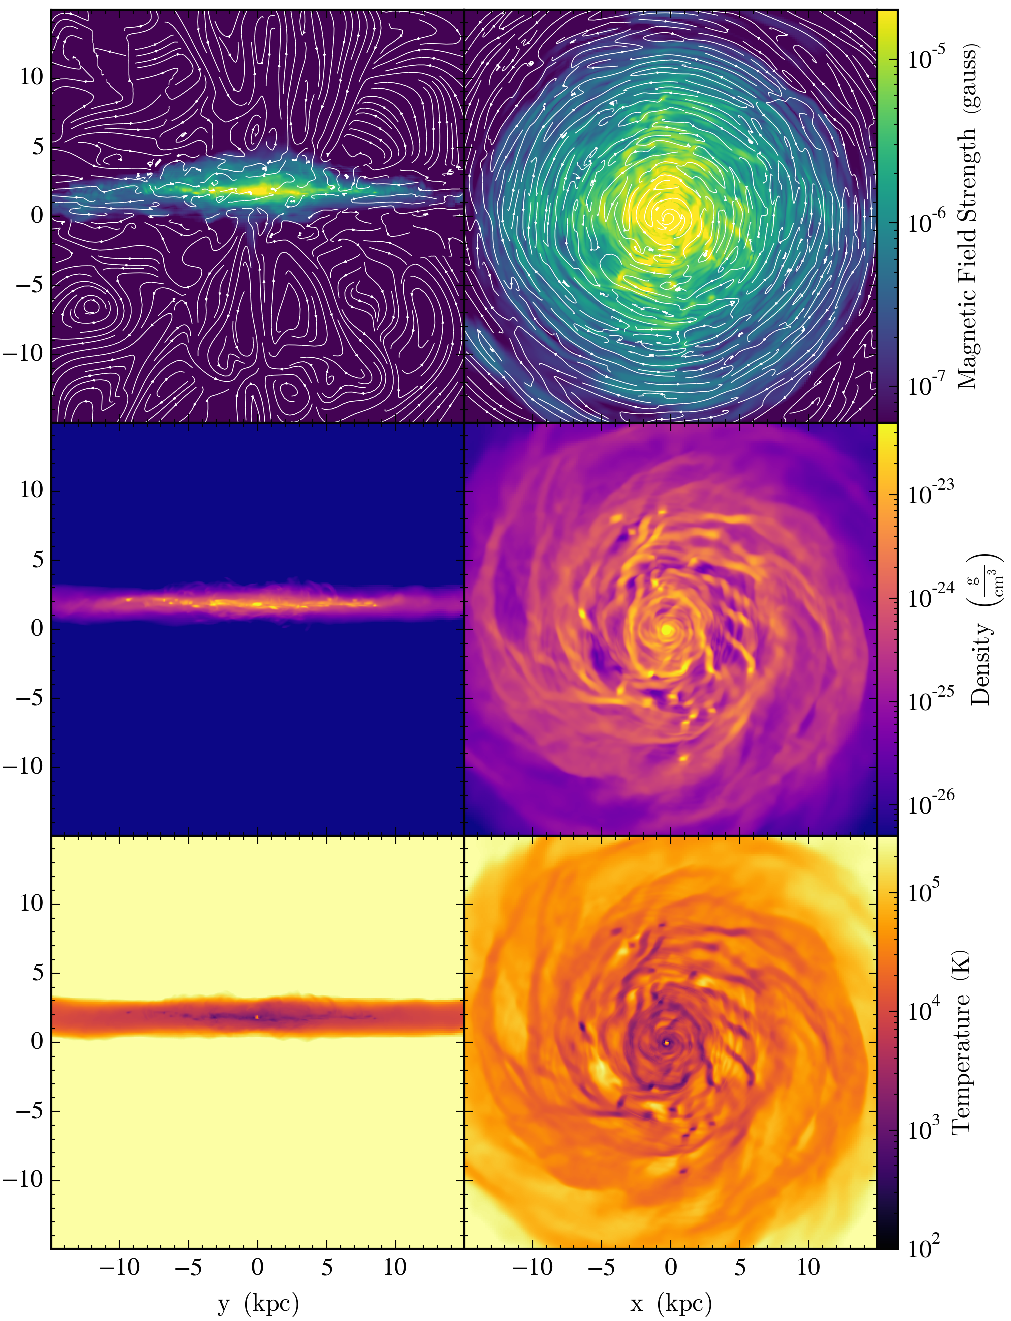
\includegraphics[width=5cm]{./images/g80_lr.pdf}
				\caption{A model at t = 2.1	Gyr in 30 kpc boxes.}
			\end{figure}
			\end{column}
		\end{columns}
\end{frame}
%====================
\begin{frame}
	\frametitle{Ab Initio Simulations of a Supernova-driven Galactic Dynamo in an Isolated Disk Galaxy \citep{2017ApJ...843..113B}}
	\begin{itemize}
		\item The main result is that a galactic dynamo can be seeded and driven by SN explosions, resulting in magnetic fields whose strength and morphology are consistent with observations.
		\item seed fields that are supplied locally, in small volumes around supernovae, can be mixed efficiently $\rightarrow$ no dramatic difference from uniform seed
		\item B attains microgauss levels over gigayear timescales throughout the disk.
		\item B develops a large-scale structure, which appears to be correlated with the disk’s spiral arm density structure
		\item seeding of the galactic dynamo by supernova ejecta predicts a persistent correlation between gas metallicity and magnetic field strength
	\end{itemize}
\end{frame}
%====================
\begin{frame}
	\frametitle{Magnetic buoyancy in simulated galactic discs with a realistic circumgalactic medium (Steinwandel et al. 2019)}
		\begin{columns}
			\begin{column}{0.48\textwidth}
				\begin{itemize}
					\item GADGET-3 code
					\item a modern version of SPH + B (SPMHD) plus resistivity and artificial viscosity and conduction terms to overcome known problems of the SPH method in terms of shock-capturing and fluid mixing instabilities (Beck et al. 2016).
				\end{itemize}
			\end{column}
			\begin{column}{0.48\textwidth}
					\begin{itemize}
						\item Powell divergence cleaning
						\item Star formation, cooling, SN feedback, and metals (Springel \& Hernquist 2003)
						\item Turbulence is driven on the scales of a few 100 pc due to SN-feedback and leads to small scale turbulent motion (similar to the $\alpha$ effect).
					\end{itemize}
			\end{column}
		\end{columns}
\end{frame}
%====================
\begin{frame}
	\frametitle{Magnetic buoyancy in simulated galactic discs with a realistic circumgalactic medium (Steinwandel et al. 2019)}
	\begin{columns}
		\begin{column}{0.6\textwidth}
			\begin{itemize}
				\item Addition of a spherical circumgalactic medium (CGM), motivated by observations and the results of cosmological simulations
			\end{itemize}
		\end{column}
		\begin{column}{0.38\textwidth}
			\begin{figure}
				\begin{center}
					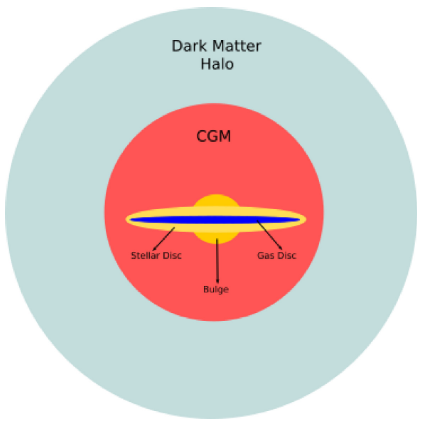
\includegraphics[width=0.8\textwidth]{./images/Steinwandel2020_galaxy_model.png}
				\end{center}
			\end{figure}
		\end{column}
	\end{columns}
\end{frame}
%====================
\begin{frame}
	\frametitle{Magnetic buoyancy in simulated galactic discs with a realistic circumgalactic medium (Steinwandel et al. 2019)}
	Two B implementation
	\begin{itemize}
		\item a primordial B of $10^{-9} \mu G$ in disk + $10^{-12} \mu G$ in CGM
		\item B is coupled to the SN explosions and seeds a magnetic dipole around an exploding star.
	\end{itemize}
	\begin{align}
	\frac{\partial \mathbf{B}}{\partial t} = \nabla \times \left( \mathbf{v} \times \mathbf{B} \right) +\eta \Delta \mathbf{B} + \left(\frac{\partial \mathbf{B}}{\partial t}\right)_\mathrm{seed}
	\end{align}
\end{frame}
%====================
\begin{frame}
	\frametitle{Magnetic buoyancy in simulated galactic discs with a realistic circumgalactic medium (Steinwandel et al. 2019)}
	\begin{columns}
		\begin{column}{0.45\textwidth}
				Strong evidence for three processes
			\begin{itemize}
				\item adiabatic compression
				\item $\alpha-\Omega$ dynamo
				\item small-scale turbulent dynamo
			\end{itemize}
		\end{column}
		\begin{column}{0.55\textwidth}
			\begin{figure}
				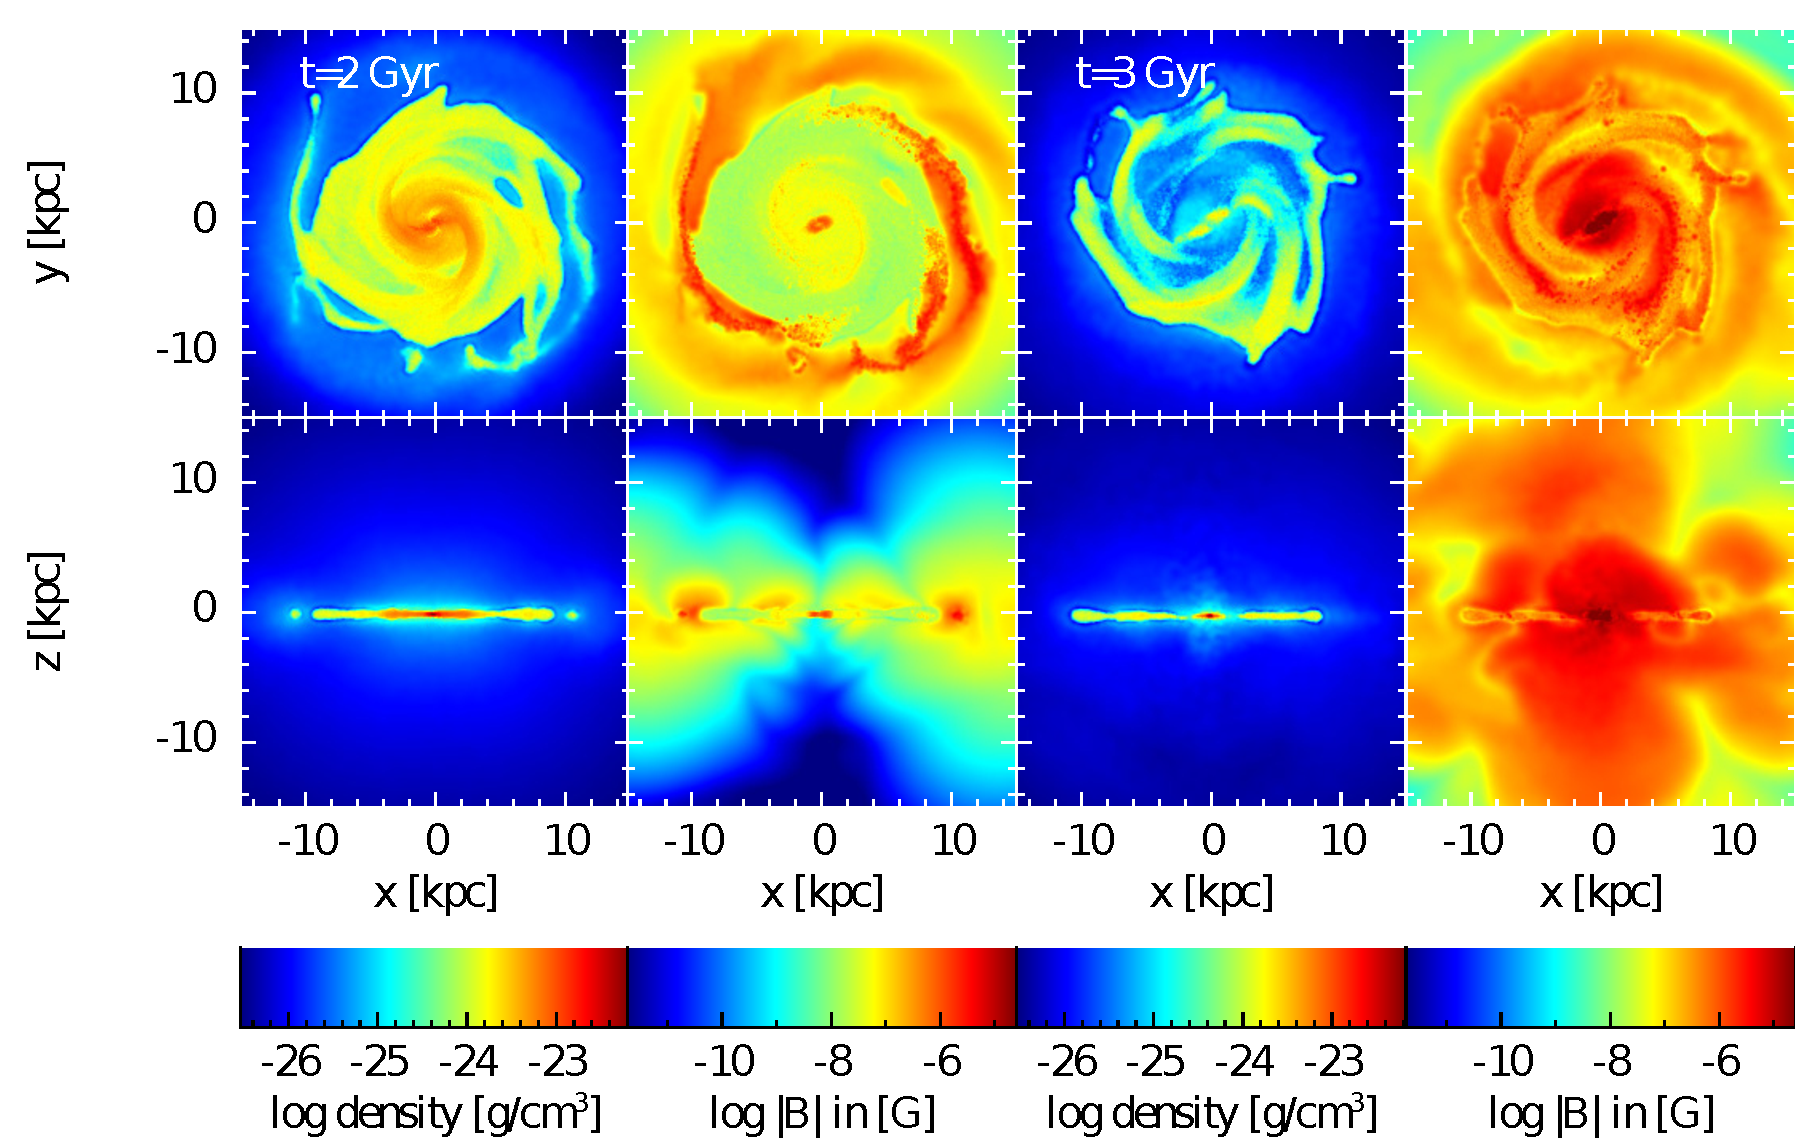
\includegraphics[width=8cm]{./images/test_seeding.pdf}
				\caption{Slice through the gas density and the magnetic field strength for the simulation MW-snB for the face-on and edge-on view. The four panels on the left-hand-side are at t = 2 Gyr, while the four panels on the right-hand-side are at t = 3 Gyr.}
			\end{figure}
		\end{column}
	\end{columns}
\end{frame}
%====================
\begin{frame}
	\frametitle{Magnetic buoyancy in simulated galactic discs with a realistic circumgalactic medium (Steinwandel et al. 2019)}
	\begin{columns}
		\begin{column}{0.52\textwidth}
				B amplification in the center of the disk leads to a biconical magnetic outflow of gas that magnetizes the CGM $\rightarrow$ 40\% reduction in SFR
		\end{column}
		\begin{column}{0.46\textwidth}
			\begin{figure}
				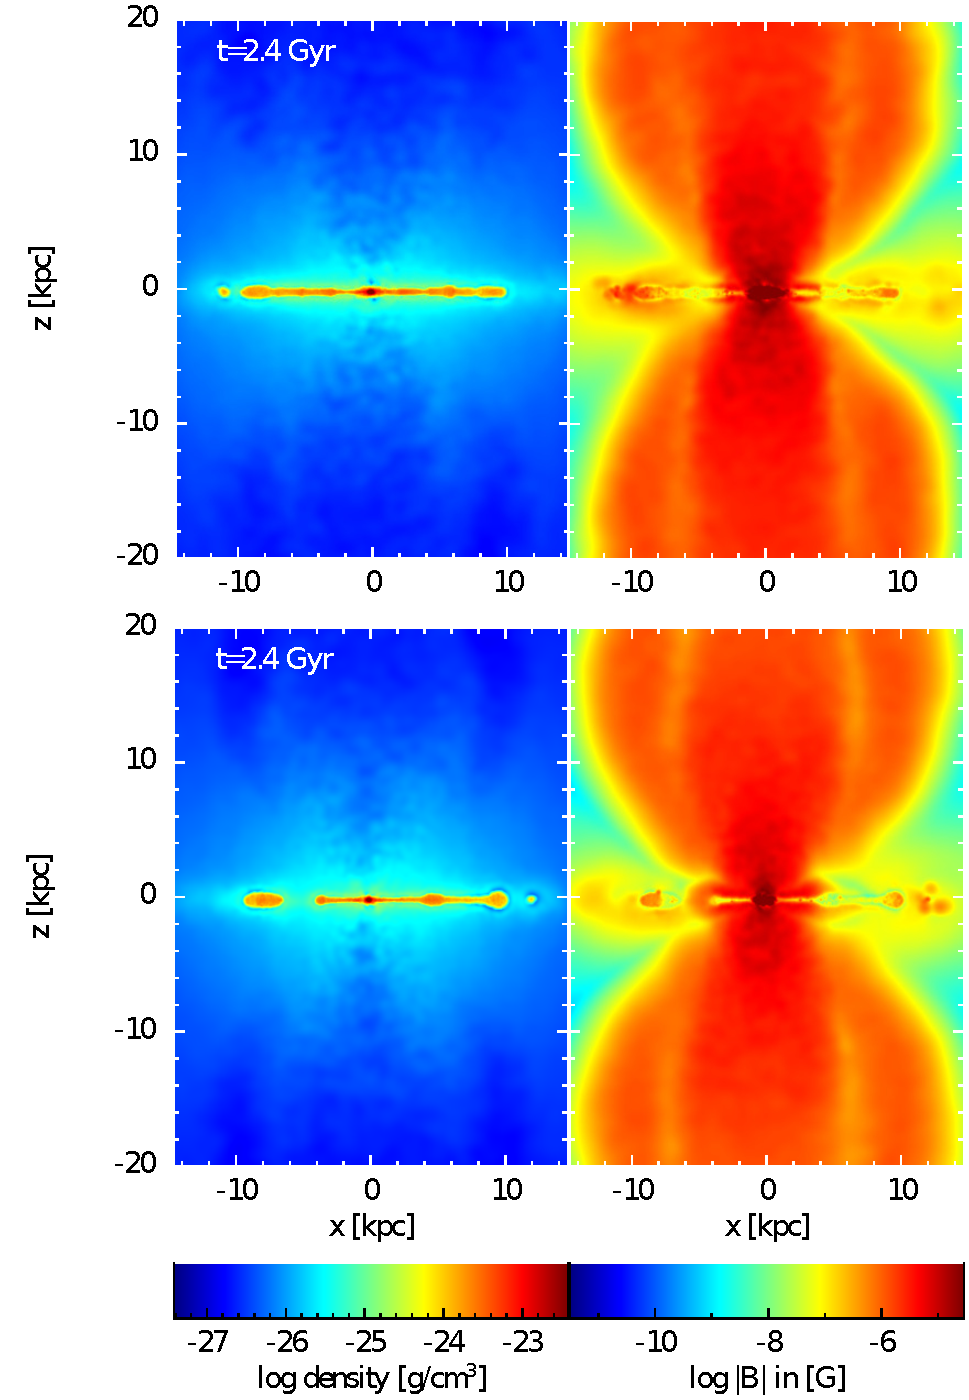
\includegraphics[width=4cm]{./images/outflow_complete.pdf}
				\caption{Cross-section slices for the MW–snB run (top panels) and the MW–primB run (bottom panels) at t = 2.4 Gyr.}
			\end{figure}
		\end{column}
	\end{columns}
\end{frame}
%====================
\begin{frame}
	\frametitle{Magnetic buoyancy in simulated galactic discs with a realistic circumgalactic medium (Steinwandel et al. 2019)}
	\begin{columns}
		\begin{column}{0.52\textwidth}
			\begin{itemize}
				\item In center, the gas density is driven by both adiabatic compression and small-scale turbulence.
				\item In spiral arms, B is lower compared to the interarm region and is amplified by adiabatic compression.
				\item In interarm regions, B is amplified by small-scale turbulence and not adiabatic compression.
				\item In outskirts of the galaxy, the amplification is not driven by adiabatic compression.
			\end{itemize}
		\end{column}
		\begin{column}{0.46\textwidth}
			\begin{figure}
				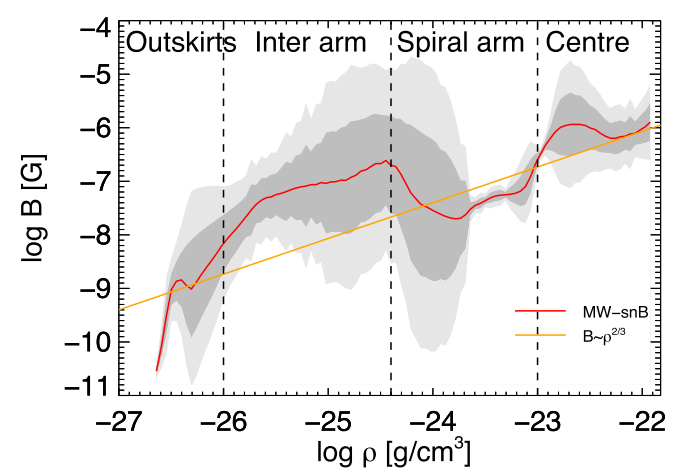
\includegraphics[width=7cm]{./images/St2019_B_rho.png}
				\caption{Median magneticfield strength for the model MW–snB}
			\end{figure}
		\end{column}
	\end{columns}
\end{frame}
%====================
%\begin{frame}
%	\frametitle{ (Steinwandel2020)}
%	\begin{center}
%		\includegraphics[width=1\textwidth]{./images/Steinwandel2020.png}
%	\end{center}
%\end{frame}
%====================
%\begin{frame}
%	\frametitle{On the origin of magnetic driven winds and the structure of the galactic dynamo in isolated galaxies (Steinwandel et al. 2020)}
%\end{frame}
%====================
\begin{frame}
	\frametitle{On the origin of magnetic driven winds and the structure of the galactic dynamo in isolated galaxies \citep{2020MNRAS.494.4393S}}
	$B\propto \Sigma_{SFR}^{1/3}$ (Schleicher $\&$ Beck; 2013)
	
	- They showed that the star formation is following the Kennicutt relation in different time.
	
	\begin{figure}
		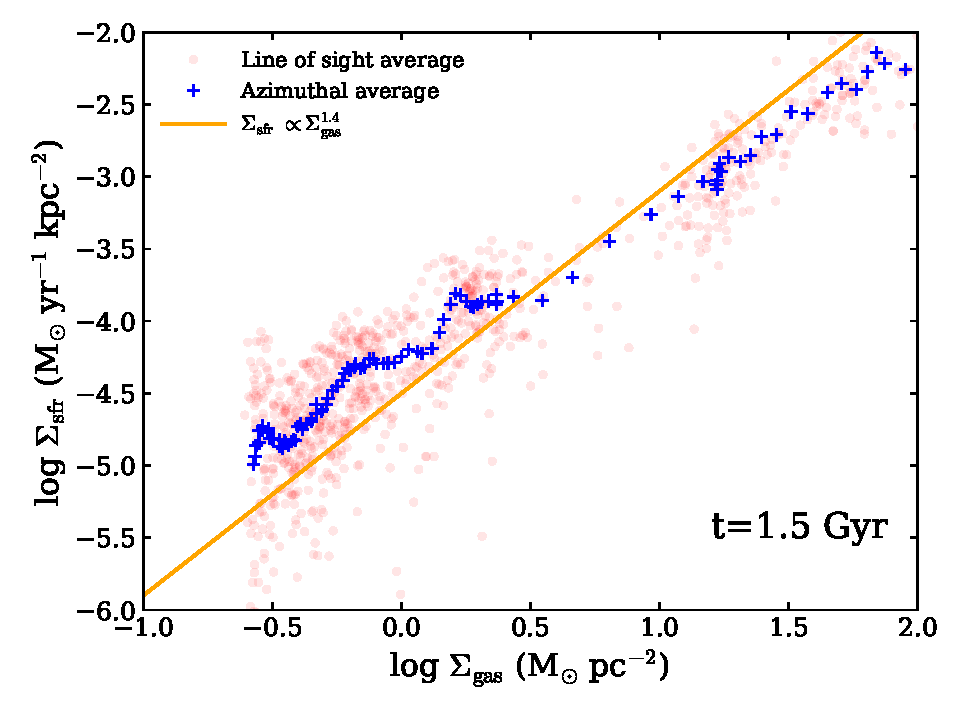
\includegraphics[width=0.5\textwidth]{./images/sk_mag_075_new.pdf}
		\caption{Star formation rate surface density as function of the gas surface density.}
	\end{figure}
\end{frame}
%====================
%\begin{frame}
%	\frametitle{ (Steinwandel et al. 2020)}
%	\begin{figure}
%		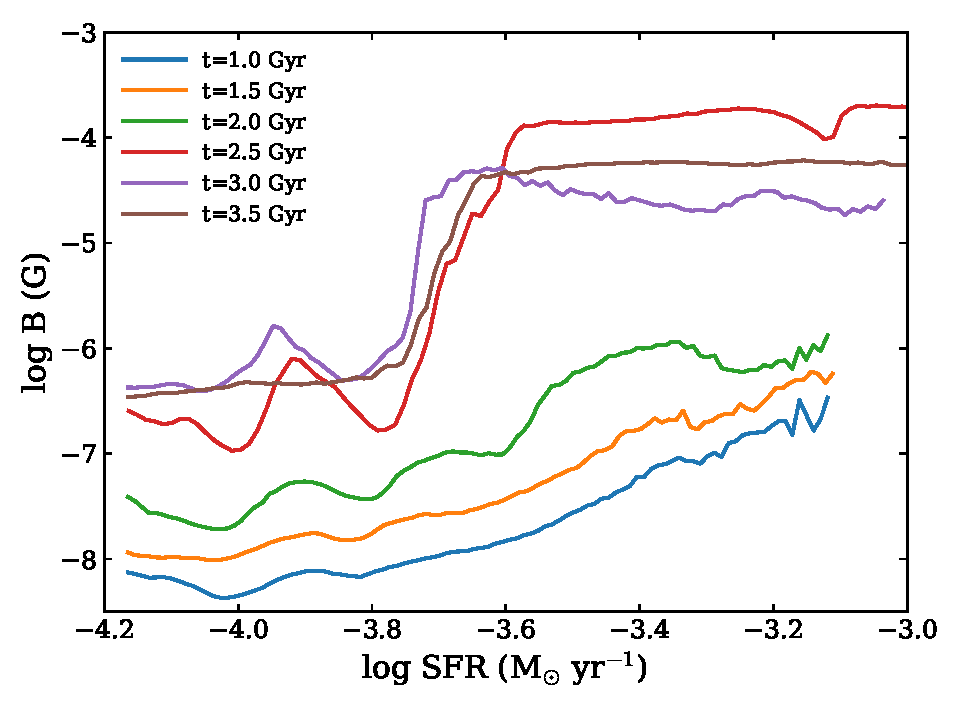
\includegraphics[width=0.75\textwidth]{./images/sfr_b_new.pdf}
%		\caption{Magnetic field as a function of the local star formation rate for six different points in time, t=$1$ Gyr (blue), t=$1.5$ Gyr (orange), t=$2$ Gyr (green),  t=$2.5$ Gyr (red),  t=$3$ Gyr (purple) and t=$3.5$ Gyr (brown).}
%	\end{figure}
%\end{frame}
%====================
\begin{frame}
	\frametitle{ On the origin of magnetic driven winds and the structure of the galactic dynamo in isolated galaxies \citep{2020MNRAS.494.4393S}}
	\begin{columns}
		\begin{column}{0.52\textwidth}
			\begin{itemize}
				\item At early times they found that B is increasing with star formation rate. However, at later points B tends to be constant as a function of the local star formation rate or is even decreasing. At intermediate time they found that the B is oscillating with increasing star formation rate which indicates that there are regions in the galaxy where the local star formation rate is increasing but B is decreasing.
			\end{itemize}
		\end{column}
		\begin{column}{0.46\textwidth}
			\begin{figure}
				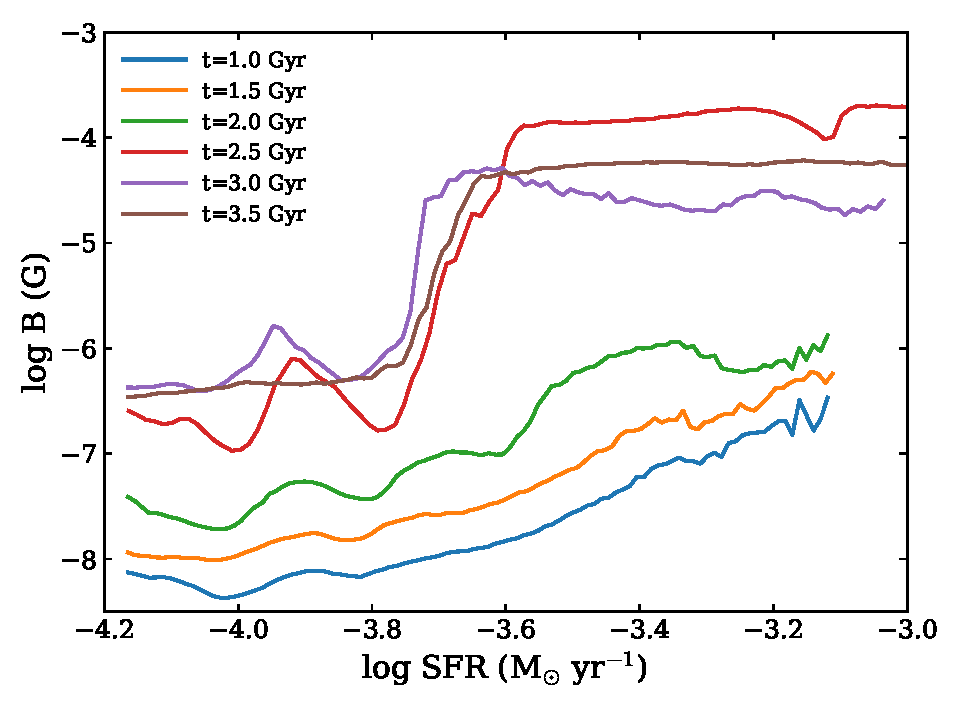
\includegraphics[width=1.1\textwidth,trim= 0 20 0 0]{./images/sfr_b_new.pdf}
				\caption{Magnetic field as a function of the local star formation rate for six different points in time, t=$1$ Gyr (blue), t=$1.5$ Gyr (orange), t=$2$ Gyr (green),  t=$2.5$ Gyr (red),  t=$3$ Gyr (purple) and t=$3.5$ Gyr (brown).}
			\end{figure}
		\end{column}
	\end{columns}
\end{frame}
%====================
\begin{frame}
	\frametitle{Discovery of massive star formation quenching by non-thermal effects in the centre of NGC 1097 \citep{2018NatAs...2...83T}}
	\begin{figure}
		\begin{center}
			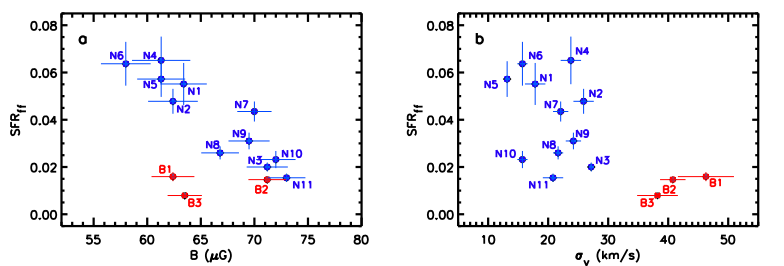
\includegraphics[width=1.\textwidth]{./images/taba2018_SFR.png}
			\caption[]{The massive SFR per free-fall, SFR$_{\rm ff}$, of the GMAs decreases with the magnetic field strength B ({\it a}) while it is uncorrelated with the turbulent velocity $\sigma_v$ ({\it b}).  The blue and red points show the narrow-  and broad-line GMAs, respectively. Strong non-circular motions/shocks in the broad-line GMAs can act as additional cause of the low SFR$_{\rm ff}$ in these clouds.}
		\end{center}
	\end{figure}
\end{frame}
%........................................................
%........................................................
\section{Example works for zoom-in simulations}
%........................................................
%........................................................
%====================
\begin{frame}
	\frametitle{Magnetic fields in cosmological simulations of disk galaxies \citep{2014ApJ...783L..20P}}	
		 For the first time the formation and evolution of a Milky Way–like disk galaxy in its \textbf{full cosmological context} while taking into account B.
		 \begin{figure}
		 	\begin{center}
		 		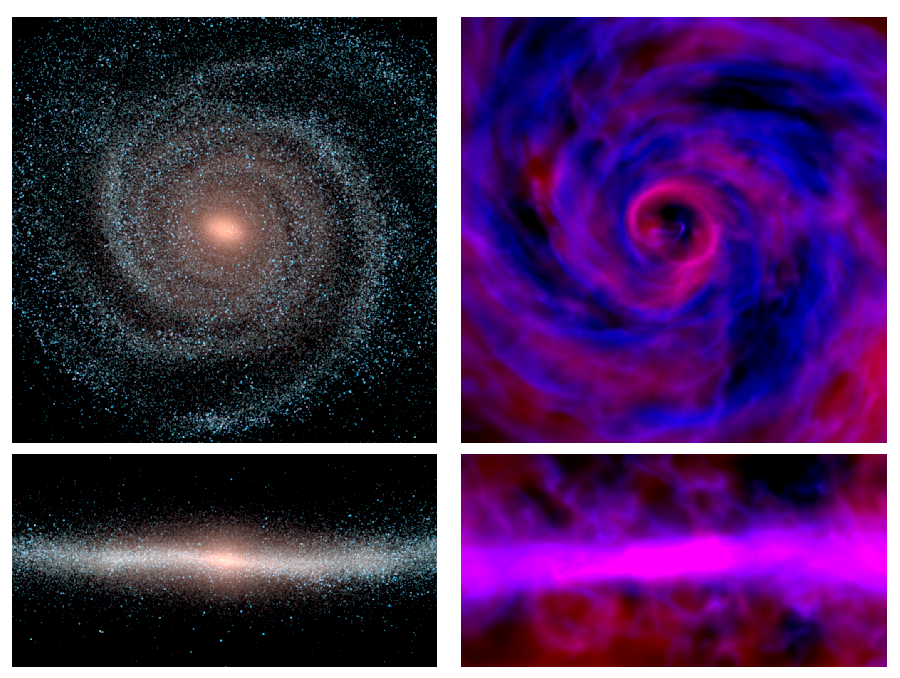
\includegraphics[width=.45\textwidth]{images/pakmor_apjl_2014/aqmhd.png}
		 		\caption{https://www.h-its.org/2014/03/10/a-milky-way-out-of-the-supercomputer}
		 	\end{center}
		 \end{figure}
\end{frame}
%====================
\begin{frame}
	\frametitle{Magnetic fields in cosmological simulations of disk galaxies (PMS14)}
	Their Baryonic physics includes (Vogelsberger et al.)
	\begin{itemize}
		\item primordial and metal line cooling
		\item a subgrid model for the inter-stellar medium (ISM) and star formation (Springel \&Hernquist 2003)
		\item a self-consistent treatment of stellar evolution and chemical enrichment
		\item galactic-scale winds (implemented with a kinetic scheme similar to Puchwein \& Springel 2013)
		\item supermassive black hole growth and feedback
	\end{itemize}	
\end{frame}
%====================
\begin{frame}
	\frametitle{Magnetic fields in cosmological simulations of disk galaxies (PMS14)}
	\begin{figure}
		\begin{minipage}[b]{0.32\linewidth}
			\centering
			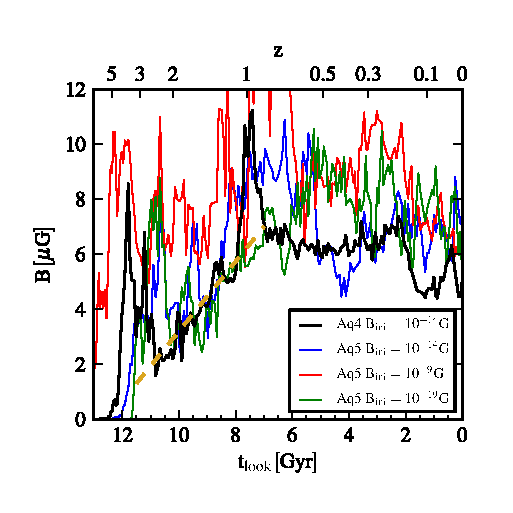
\includegraphics[width=\textwidth]{images/pakmor_apjl_2014/bfield_evol_Aq-A_4}
		\end{minipage}
		\begin{minipage}[b]{0.32\linewidth}
			\centering
			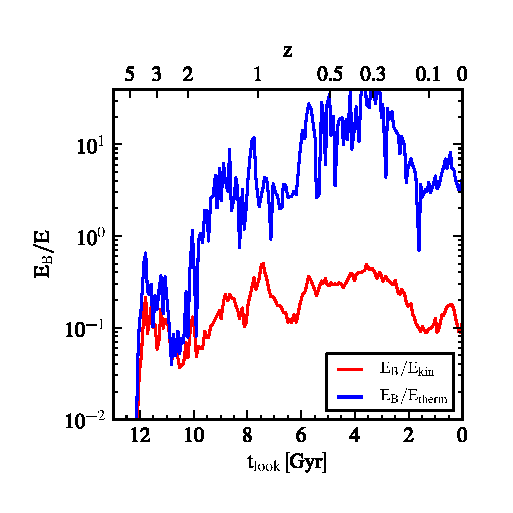
\includegraphics[width=\textwidth]{images/pakmor_apjl_2014/energyrel_evol_Aq-A_4}
		\end{minipage}
		\caption{Evolution of the volume weighted average root mean square magnetic field strength (right), the ratio of magnetic energy to kinetic energy and thermal energy (left).}
	\end{figure}
	\begin{itemize}
		\item<1|only@1> They found that a prescribed tiny magnetic seed field \textbf{grows exponentially} by a small-scale dynamo until it saturates around z = 4 with a magnetic energy of about $10\%$ of the kinetic energy in the center of the galaxy's main progenitor halo.
		\item<2|only@2> By z=2, a well-defined gaseous disk forms in which B is further \textbf{amplified} by differential rotation, until it saturates at an average field strength of $\sim 6 \mu G$ in the disk plane.
		\item<3|only@3> In this phase, B is transformed from a chaotic small-scale field to an \textbf{ordered} large-scale field on scales comparable to the disk radius.
		\item<4|only@4> They suggested that the \textbf{large-scale B in spiral galaxies} can be explained as a result of the \textbf{cosmic structure formation} process.
	\end{itemize}
\end{frame}
%====================
\begin{frame}
	\frametitle{Effects of simulated cosmological magnetic fields on the galaxy population\\ \citep{2016MNRAS.456L..69M}}	
	They examine 
	\begin{itemize}
		\item how strong the effects of cosmological
		B fields (i.e. fields generated in the early Universe) on the global properties of the galaxy population are as a function of the field strength
		\item what is the critical intensity at which they become noticeable
	\end{itemize}
	Baryonic physics as Pakmor et al. (2014)
\end{frame}
%====================
\begin{frame}
	\frametitle{Effects of simulated cosmological magnetic fields on the galaxy population (MV16)}	
	\begin{figure}
		\begin{minipage}[b]{0.35\linewidth}
			\centering
			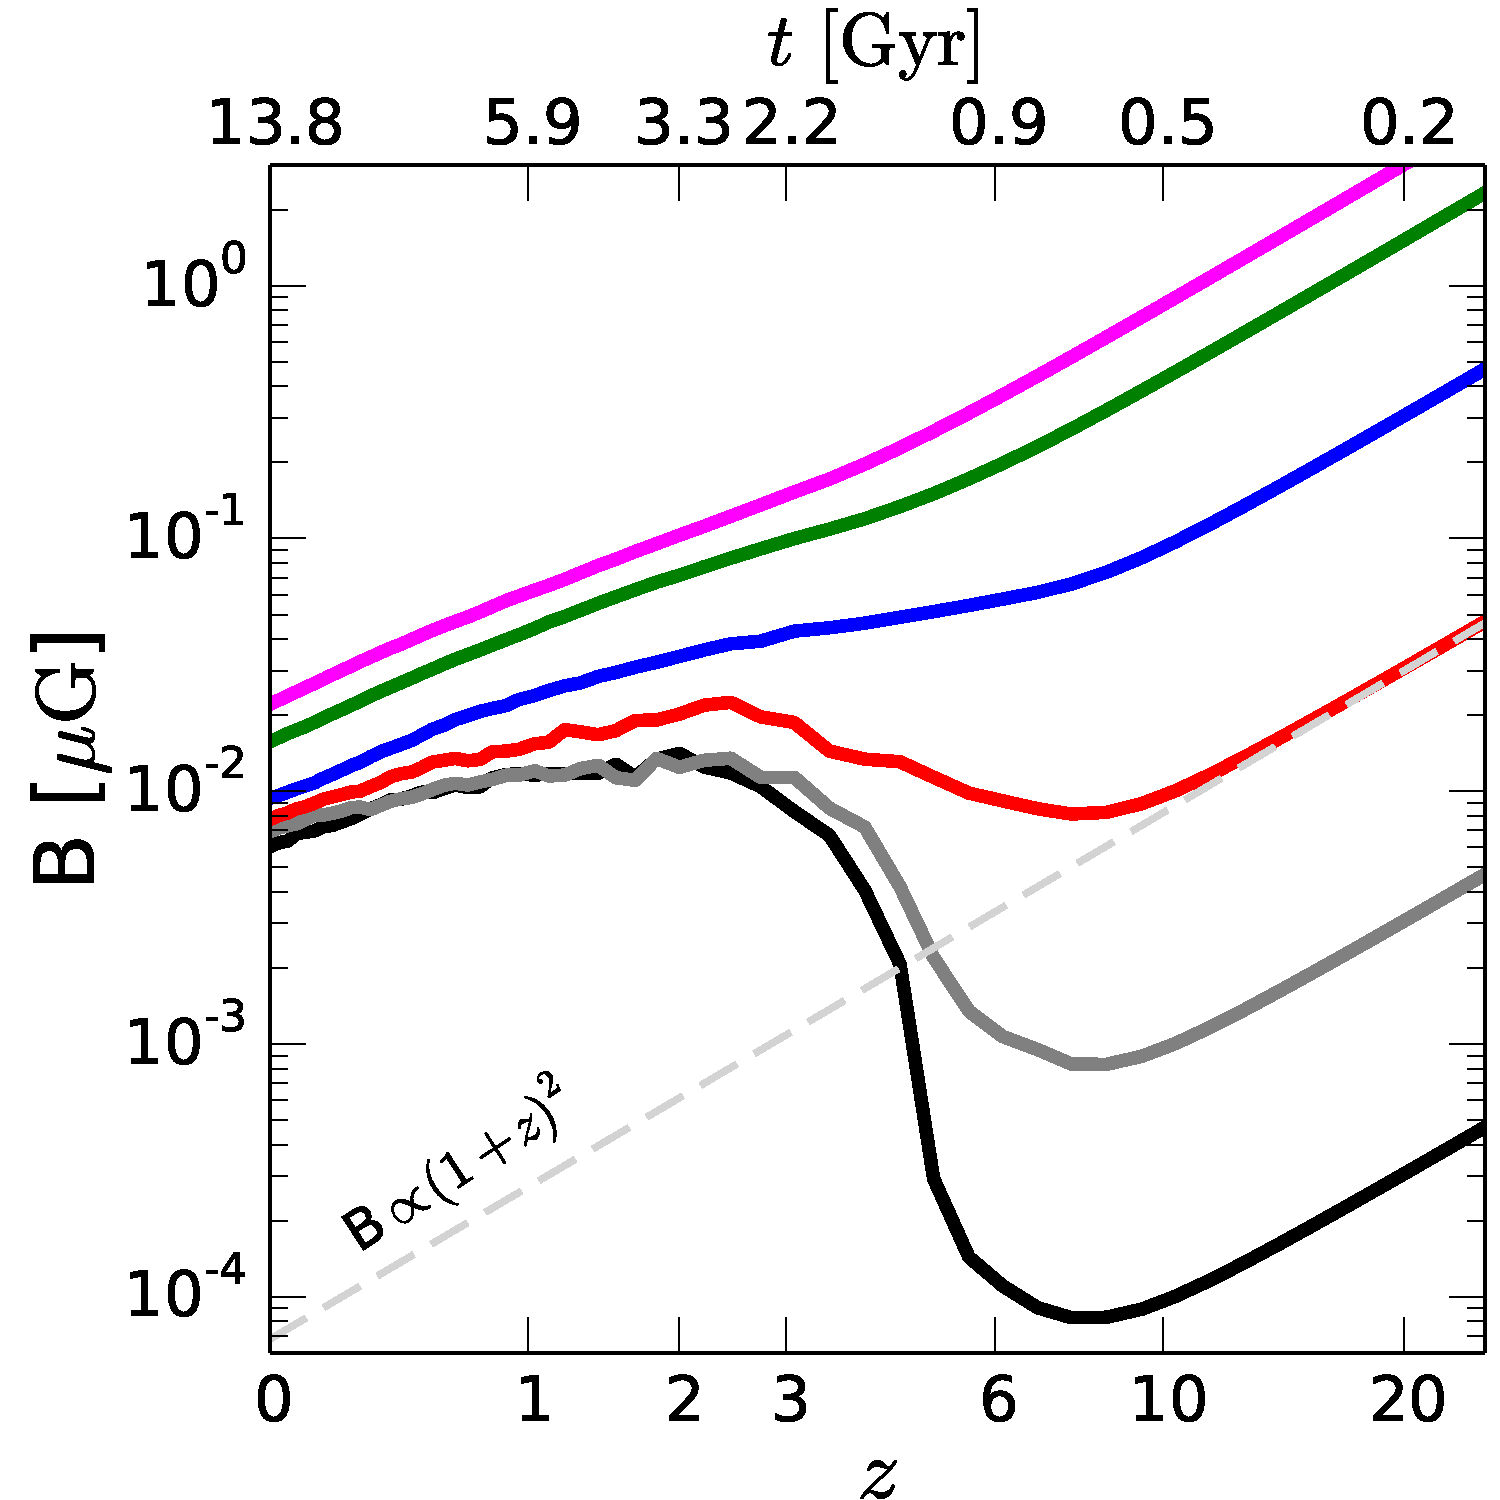
\includegraphics[width=\textwidth]{images/marinacci_2016/fig1a.pdf}
		\end{minipage}
		\begin{minipage}[b]{0.35\linewidth}
			\centering
			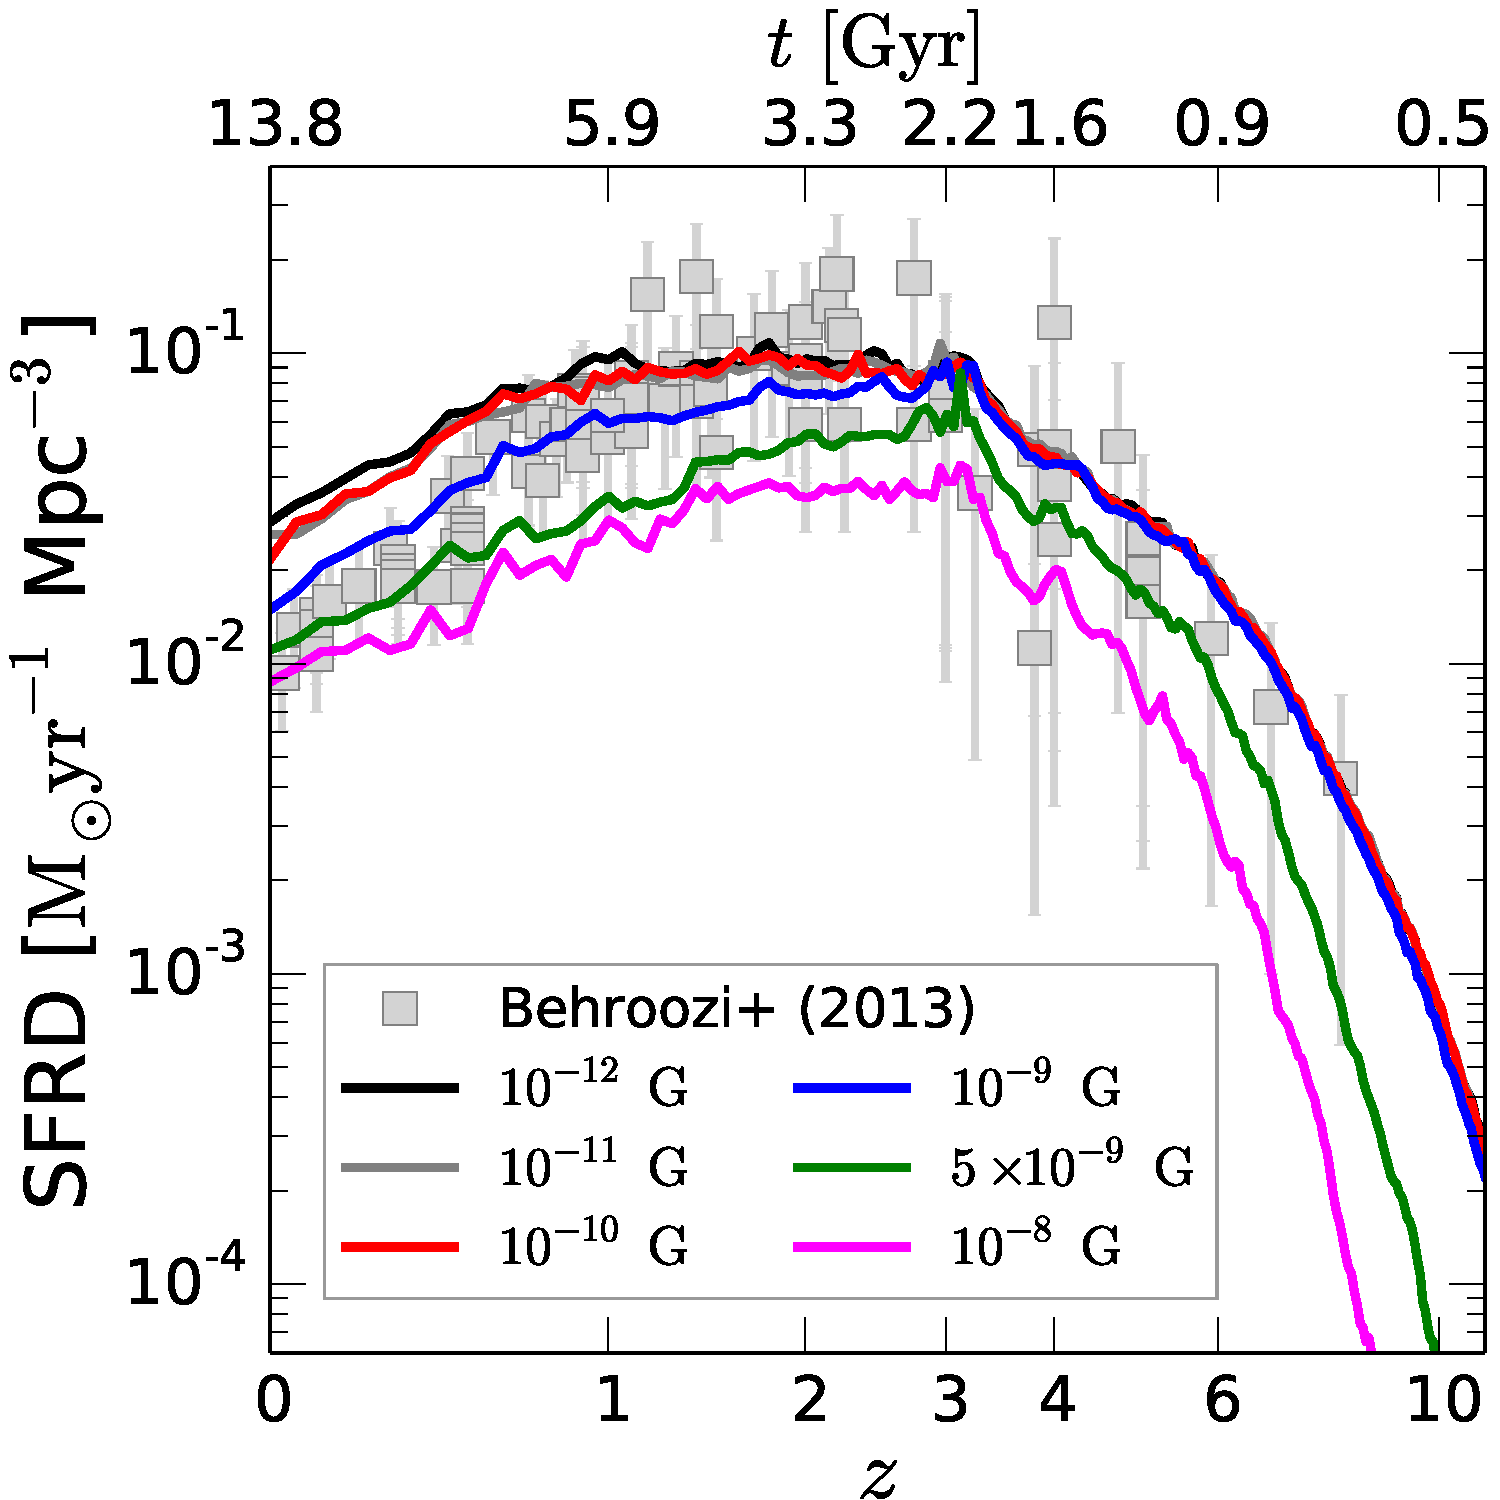
\includegraphics[width=\textwidth]{images/marinacci_2016/fig1b.pdf}
		\end{minipage}
		\caption{Evolution of the volume-weighted rms B field 
			strength (left) and cosmic star formation rate density (SFRD) 
			together with  a compilation of observational data (right)
		}
	\end{figure}
	\begin{itemize}
	\item<1|only@1> Above the \textbf{critical B} field value of $10^{-9}\,G$, the field intensity is \textbf{set by flux conservation} and little turbulent amplification is present.
	\item<2|only@2> For \textbf{larger seed} magnetic field strengths there is an \textbf{increasing suppression} of the SFRD, which is present at all times for seed 
	fields $>10^{-9}\,G$.
\end{itemize}
\end{frame}
%====================
\begin{frame}{Bibliography}
		\bibliographystyle{aasjournal}
		\bibliography{references}
\end{frame}


\end{document}
